%************************************************
\chapter{Social Media Specific Approaches}\label{ch:saosm}

%************************************************

Since social networks posed special problems in sentiment analysis, it became important to come up with special approaches to deal with them. Ever since the sentiment analysis
research on social media started, researchers have been trying to combat these problems by suggesting approaches and coming up with the tools that are more suited to this domain.
We know that, in a classification-problem setting of sentiment analysis problem, the choice of features play the most important role. Since the characteristics of social media
text are very much different from regular plain English (or any other) text, the features would have to be re-engineered. This is only one of the many adaptations that our
sentiment analysis systems have to undergo if they have to be applied to social networks. 

\vspace{8mm}

Redesign of features, however, is not enough. We know that NLP tools have always been of great help when it comes to sentiment analysis. Tools like lexicons, wordnets, parsers etc. have
greatly contributed to the design of sentiment analysis systems. The problem is, these tools fail miserably when applied to social networks. What we need is a redesigning of these
tools as well, so as to make it suitable to our domain of interest, or to come up with alternative approaches.


\section{Classification Features}

To understand what features are important for sentiment classification in social media domain, one needs to know about the practices and conventions of modern social networking.
One cannot afford to be ignorant to the hieroglyphs and the abbreviations that the users are generating everyday if he/she really wants to understand their sentiments.
The state-of-the-art system in Tweet Sentiment Analysis, NRC-Canada have used the following features in their system: \cite{saif}

\begin{enumerate}
\setlength{\itemsep}{15pt}
 \item \textbf{Word ngrams and Character ngrams:} Character n-grams are added specially because word n-grams are not always useful to capture the language (because of frequent misspelling)
 \item \textbf{All caps, Elongated words and Punctuations:} These have special meaning in social networks. All caps are used to denote 'yelling' or abbreviations, both of which are useful
 for sentiment analysis. Elongated words (also called intensifiers) are diligent misspellings of known words to emphasize on their emotions. Punctuations also
 perform the same function. They are not cameos of language grammar here in this context. A lot of repeated punctuations (question or exclamation) is a very often sight 
 in social media, which denotes intensity of emotion.
 For example, \textbf{OMG I am soooo happy!!!!!!!!}
\item \textbf{POS tags:} Using POS tags as a feature is not new to social media. However, the regular POS tagger can't be used here, rather a special tool created by Carnegie Mellon
is used.
\item \textbf{Negation:} The number of negated contexts in the text. It has been shown that if we handle negation well, we can increase the sentiment accuracy to a great extent.
\item \textbf{Hashtags and Emoticons:} These are the most powerful features that social networks have to offer. Emoticons, most of the times, very much sum up the emotion of
the text they are contained in (of course, only if the author knows how to use them correctly) whereas hashtags act as predefined labels that automatically put the text in some
class of tweets. We can then, find the polarity of the hashtag and it is very much likely that this will be the polarity of the given text.
\item \textbf{Lexicon features:} Lexicon features make use of a pre-built lexicon that contains sentiment scores of various phrases. Here, we look for things like the number
of words in the text with a positive score in the lexicon, or the average score of the text, as given by summation of individual scores of all phrases obtained from the lexicon etc.

\end{enumerate}

These kind of features, on an SVM classfier have successfully given an accuracy as high as 88.93\% over tweets.
\section{Dependency Parser for Tweets}

As already discussed, NLP tools have alwyas been very helpful in sentiment analysis. One such tool is the dependency parser. As is true for most of NLP techniques, this also
cannot be used directly in social network domain. In this section, we will see why. Also, the adaptations that need to be made are discussed. \cite{tweebo}

\subsection{Challenges}

\begin{enumerate}
\setlength{\itemsep}{15pt}
 \item Tokens may or may not have syntactic functions. So, their identification is important. Consider this:
 \vspace{8mm}
 
 \textbf{Another fine effort from @IamRaina}
 
 \vspace{8mm}
 
 The token @IamRaina is a part of the sentence structure and hence has a syntactic function. On the other hand, in the example to follow, the same token does not have a 
 syntactic function.  
 
 \vspace{8mm}
 
 \textbf{Suresh Raina has always been agile on the field and hard hitting with the bat. @IamRaina}
 
 \item Internal analysis of Multi-word Expressions [MWE] is not very important for the task at hand. Annotators should not expend energy on developing and respecting conventions (or making
arbitrary decisions) within syntactically opaque units. e.g. World Cup 2015 (Proper Nouns), as well as (Connectives), out of (Prepositions) etc.
\item Tweets need not be a single sentence. They may contain multiple utterances, each with its syntactic root
disconnected from the others.
\item Noun phrase internal structures are usually poorly represented by most parsers. Richer treatment of such structures is required in the dependency parser we seek
to design. For example, the phrase \textquotedblleft
Cricket World Cup Final Match\textquotedblright will have the constituency parse tree as shown above.

\begin{figure}[t]
\centering
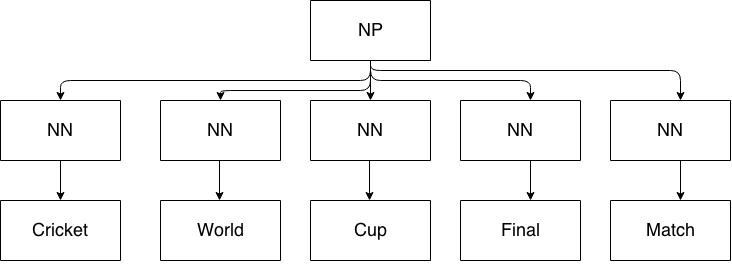
\includegraphics[scale=0.4]{gfx/parse.png}
\caption{A Constituency Parse }
\end{figure}
\vspace{8mm}
This when converted to a dependency parse will generate something like Figure 4.
\begin{figure}[t]
\centering
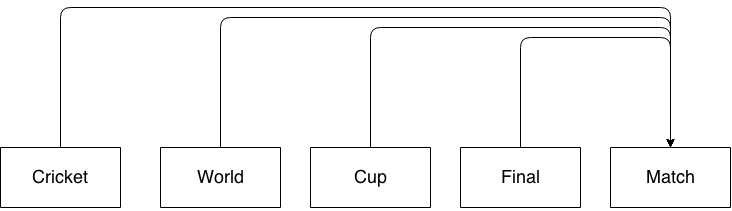
\includegraphics[scale=0.4]{gfx/parse2.png}
\caption{Equivalent Dependency Parse }
\end{figure}

 \vspace{8mm}
 
 However the accurate representation of the dependency parse should be as given in Figure 5.
 
 \begin{figure}[t]
\centering
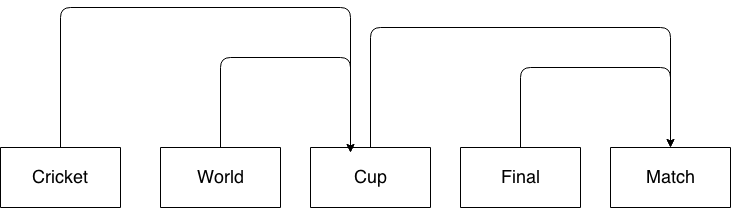
\includegraphics[scale=0.4]{gfx/parse3.png}
\caption{The richer dependency parse }
\end{figure}
 
\end{enumerate}

\subsection{Design of the dependency parser}

This section deals with how the traditional dependency parsing algorithm is adapted for tweet dependency parsing. 
The required parse tree is given by the following formula:

\begin{framed}
 \begin{equation*}
Parse^\star(x) = argmax_{y \epsilon Y_x} W^T g(x, y)
\end{equation*}
\end{framed}

where, 


\begin{itemize}
\item x : input sentence \\
\item $Y_x$ : Set of all possible dependency parses of x \\
\item g : feature vector representation \\
\item W : parameter vector of weights, learnt by data
\end{itemize}

Decomposition of features into parts is critical to the performance of the parser. Let us consider there are n different tokens in our sentence. Then, the set of all possible dependency
arcs is given by $A = {(h,m) : h  \epsilon (0,n), m  \epsilon (1,n)}$ 

\vspace{8mm}

Then, Y, the set of all dependency parses is given as $Y \subset (0,1)^{|A|}$. $g$ can be decomposed into features over each branch in the dependency parse. For example, consider:
\begin{framed}
 \begin{equation*}
very \leftarrow good \leftarrow food
\end{equation*}
\end{framed}

$g(x,y)$ can be calculated as $score(good \rightarrow very) + score(food \rightarrow good)$. Now, $score(w_h,w_m)$ is given as a weighted sum of score over individual features.

\begin{framed}
 \begin{equation*}
score(w_h \rightarrow w_m) = \phi (x, <h,m>) \theta
\end{equation*}
\end{framed}

Here $\phi$ is a feature vector and $\theta$ is the vector of weights.
\section{Exploiting the social graph}

So far in this report, all problems in sentiment analysis were tackled at the document level or aspect level (thearting). However, user level sentiment analysis is equally 
important and interesting. Moreover, it is easier to perform since we are making a bold assumption that a user always tweets with the same sentiment. This is not true in practice.
But when we restrict our domain to a specific topic, this type of behaviour is known to emerge. For example, if a person is inclined towards or associated with an organization,
he will mostly (if not always) talk positively about that particular organisation. Thus, user level sentiment analysis becomes valid.

\vspace{8mm}

The approach of using the social graph to determine user sentiments is based on a psychological principle called \textquotedblleft homophily\textquotedblright. There is a 
popular phrase in English that defines the underlying idea - \textquotedblleft Birds of a feather flock together.\textquotedblright  In sentiment analysis, this would mean
that people who interact more on a social network among each other are likely to hold a similar sentiment on a particular topic. Of course, for this approach to work, we need
to start with some seed set of people whose sentiments are already known. \cite{user}

\vspace{8mm}

In a Twitter environment, the relationship between users can be extracted in the form of four different graphs:

\begin{enumerate}
\setlength{\itemsep}{15pt}
\item Directed follow graph: user $v_i$ follows $vj$ ( $v_j$ may or may not follow $v_i$ in return )
\item Mutual follow graph: user $v_i$ follows $v_j$ and user $v_j$ follows $v_i$
\item Directed @ graph: $v_i$ has mentioned $v_j$ via a tweet containing @$v_j$ ( $v_j$ may or may not mention $v_i$ in return )
\item Mutual @ graph: $v_i$ has mentioned $v_j$ via a tweet containing @$v_j$ and vice versa

\end{enumerate}

\begin{figure}[t]
\centering
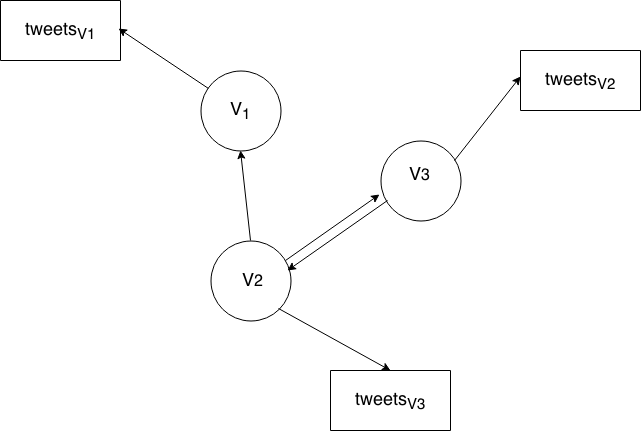
\includegraphics[scale=0.4]{gfx/graph.png}
\caption{A sample directed follow graph}
\end{figure}

Let us assume the number of users be V. Let $y_{v_i}$ be the label for
user $v_i$, and Y be the vector of labels for all users. We make
the Markov assumption that the user sentiment $y_{v_i}$ is influenced only by the sentiment labels of tweets belonging to that particular user and the sentiment labels
of the immediate user neighbors. 
\vspace{8mm}

Probability of a particular Y vector will be given as:

%\setlength{\fboxsep}{10pt}
%\setlength{\fboxrule}{5pt}
%\fbox{A frame.}

 \begin{equation*}
log P(Y) = \sum_{v_i \epsilon V} \left( \sum_{t \epsilon tweets_{v_i}} \mu_{k,l} f_{k,l} (y_{v_i}, y_t) + \\ \sum_{v_j \epsilon neighbours_{v_i}} \lambda_{k,l} h_{k,l} (y_{v_i}, y_{}) \right)
\end{equation*}

where,

\vspace{8mm}

indices k, l range over the set of sentiment labels (0,1). \\
$f_{k,l}$ and $h_{k,l}$ are feature functions, and $\mu_{k,l}$ and $\lambda_{k,l}$ are parameters representing impact. \\
Z is the normalization factor

\vspace{8mm}

We can keep changing f,h,$\mu$ and $\lambda$ to meet different kind of adaptation needs. For example, $f_{k,l} (y_{v_i}, y_t)$ will fire only if $y_{v_i} = k$ and $y_t = l$.
Even after that, we can have different values of f depending upon whether $v_i$ is a labeled user or not. We can also tweak $\mu$ as $\mu_{1,0}=0$. This means that we are giving 
no weightage to the case where a positively labeled user posts a negative tweet. (Assuming 1 as positive and 0 as negative.)







